\section{Auswertung}
Die Auswertung, genauer die Fehlerrechnung, die Plots und Ausgleichsrechnung erfolgt mit den Paketen
Numpy \cite{numpy}, Uncertainties \cite{uncertainties}, Matplotlib \cite{matplotlib} und Scipy \cite{scipy} in der Programmiersprache python.
\subsection{Fehlerrechnung}
Die Mittelwerte werden nach
\begin{equation}
	\bar{x}=\frac{1}{N}\sum_{i}^N x_i
\end{equation}
und deren Standardabweichung mit
\begin{equation}
	\sigma_{\bar{x}} = \sqrt{\frac{1}{N(N-1)} \sum_{i}^N (x_i-\bar{x})^2}
\end{equation}
berechnet.
Für die Fehlerfortpflanzung einer Variablen $x_i$ gilt
\begin{equation}
	\sigma = \sqrt{\sum_{i}^N \Bigl(\frac{\partial f}{\partial x_i} \sigma_{x_i}\Bigr)^2}.
	\label{eq:gaussfehler}
\end{equation}
Als Fehler für die Messgeräte, das Amp\`{e}re-, das Volt- und das Ohm-Meter, wird ein Fehler von $\pm 1$ auf die erste Nachkommastelle angenommen;
als Reaktions- und Ablesezeit wird mit einem Fehler von $\SI{3}{\second}$ gerechnet.

\subsection{Bestimmung der Molwärme von Kupfer}

Um die Wärmekapazität $C$ eines Festkörpers zu berechnen, ist es nötig, die Wärmemenge $\delta Q$ zu kennen.
Sie wird aus den gemessenen Strom-Spannungs-Paaren und der Zeit pro Messwertnahme durch
\begin{equation}
  \delta Q = U I \delta t
\end{equation}
berechnet und in
\begin{equation}
  C=\frac{\delta Q}{n\delta T}
\end{equation}
eingesetzt.
Durch den linearen Zusammenhang zwischen dem gemessenen Widerstand $R$ und der Temperatur $\delta T$
\begin{equation}
  T=\SI{0,00134}{\frac{K}{\ohm^2}} R^2 + \SI{2,296}{\frac{K}{\ohm}} R - \SI{243,02}{K}
\end{equation}
wird das $\delta T$ zur Molwärme berechnet.\\
Wird die Molwärme für eine Stoffmenge $n= \frac{m}{M}$ und anstelle eines konstanten Volumens bei einem festen Druck $p$ betrachtet,
so folgt
\begin{equation}
  C_p=\frac{MUI\delta t}{m\delta T}.
\end{equation}
Die Masse des Kupferwürfels ist mit $m=\SI{0,342}{kg}$ angegeben \cite{anleitung}.
Ferner wird mit einer morlaren Masser für Kupfer von $\SI{63,546}{u}$ gerechnet \cite{molaremassecu}.\\

Die Umrechnung von $C_P$ in $C_V$ erfolgt mit
\begin{equation}
  C_V = C_P-9\alpha ^2 \kappa V_0 T.
\end{equation}
Benötigt werden hierfür der Kompressionsmodul $\kappa$, der für Kupfer durch $\kappa= \SI{140}{\frac{GN}{m^2}}$ gegeben ist, auch das molare Volumen $V_0$,
\begin{equation}
	V_0=\frac{M}{\rho}=\SI{7,092}{\frac{m^3}{\symup{mol}}}
\end{equation}
mit der molaren Masse $M$ und der Dichte von Kupfer $\rho=\SI{8,96}{\frac{g}{cm^2}}$\cite{molaremassecu}.\\
Der temperaturabhängige lineare Ausdehnungskoeffizient $\alpha$ wurde mit den aus \cite{anleitung} zugehörigen Temperaturwertepaaren durch eine Funktion
\begin{equation}
	\alpha(T)=\frac{x}{T}+y
\end{equation}
gefittet. Der lineare Zusammenhang und das Ergebnis der Regression ist in Abbildung \ref{fig:alphaplot} zu sehen.

\begin{figure}[H]
  \centering
  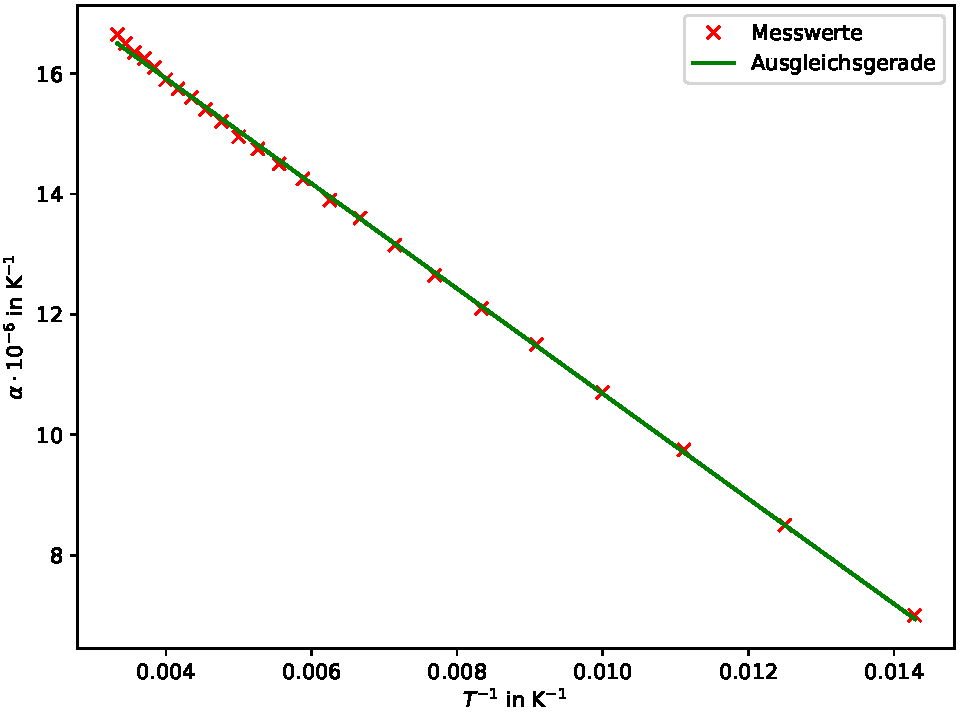
\includegraphics[width=0.9\textwidth]{plots/alphaplot.pdf}
  \caption{Linearer Zusammenhang des Ausdehnungskoeffizienten $\alpha$ gegen die inverse Temperatur $\frac{1}{T}$.}
  \label{fig:alphaplot}
\end{figure}

Die Regression liefert folgende Zahlenwerte für die beiden Parameter $x$ und $y$:
\begin{align*}
	x &=(-873 \pm 4)\cdot 10^{-6}\\
	y &=\SI{19,41 \pm 0,03}{\frac{1}{K}}
\end{align*}
Im Folgenden findet die Berechnung aus den Messwerten der Molwärme bei konstantem Druck $C_P$ und die daraus abgeleitete Molwärme bei konstantem Volumen $C_V$
nach den oben genannten Formeln statt. Alle Messwerte des Versuchs sowie die errechneten Größen $T$, $C_P$ und $C_V$ befinden sich in Tabelle \ref{tab:wertegesamt}.



\begin{table}[htb]
  \centering
  \caption{Gemessene und berechnete physikalische Größen zur Bestimmung der
  molaren Wärmekapazität einer Kupferprobe.}
  \begin{tabular}{S[table-format=2.2,separate-uncertainty,table-figures-uncertainty=1]
                  S[table-format=2.2,separate-uncertainty,table-figures-uncertainty=1]
                  S[table-format=2.2,separate-uncertainty,table-figures-uncertainty=1]
                  S[table-format=2.2,separate-uncertainty,table-figures-uncertainty=1]
                  S[table-format=2.2,separate-uncertainty,table-figures-uncertainty=1]
                  S[table-format=2.2,separate-uncertainty,table-figures-uncertainty=1]}
      \toprule
      {$\delta t$ in \si{\second}} & {$R$ in \si{\ohm}} & {$I$ in \si{\milli\ampere}} & {$U$ in \si{\volt}} & {$T$ in \si{\kelvin}} & {$C_{\mathrm{P}}$ in \si{\joule\per\mol\per\kelvin}} \\
      \midrule
      0(0)  & 22,0(1) & 150,5(1) & 13,27(1) & 81.29(24)&	0(0)\\
      302(3)& 26,2(1) & 153,1(1) & 13,27(1) & 91.21(24)&	11,5(4)\\
      250(3)& 30,0(1) & 154,2(1) & 13,26(1) & 100.22(24)&	10,5(4)\\
      300(3)& 33,3(1) & 154,8(1) & 13,25(1) & 108.07(24)&	14,6(6)\\
      330(3)& 37,0(1) & 164,0(1) & 13,28(1) & 116.92(24)&	15,1(6)\\
      300(3)& 40,8(1) & 173,8(1) & 13,30(1) & 126.04(24)&	14,1(5)\\
      300(3)& 44,4(1) & 170,3(1) & 13,29(1) & 134.71(24)&	14,6(6)\\
      300(3)& 48,0(1) & 178,5(1) & 13,32(1) & 143.43(24)&	15,2(6)\\
      300(3)& 51,7(1) & 181,5(1) & 13,33(1) & 152.41(24)&	15,0(6)\\
      300(3)& 55,4(1) & 186,3(1) & 13,34(1) & 161.44(24)&	15,3(6)\\
      300(3)& 59,3(1) & 186,6(1) & 13,34(1) & 170.99(25)&	14,5(5)\\
      300(3)& 63,1(1) & 186,8(1) & 13,35(1) & 180.34(25)&	14,9(6)\\
      300(3)& 66,7(1) & 186,9(1) & 13,35(1) & 189.23(25)&	15,6(6)\\
      300(3)& 70,3(1) & 187,0(1) & 13,35(1) & 198.16(25)&	15,6(6)\\
      300(3)& 73,8(1) & 188,9(1) & 13,36(1) & 206.87(25)&	16,2(7)\\
      300(3)& 77,5(1) & 189,1(1) & 13,37(1) & 216.12(25)&	15,2(6)\\
      300(3)& 81,1(1) & 189,3(1) & 13,37(1) & 225.15(25)&	15,6(6)\\
      300(3)& 84,3(1) & 189,4(1) & 13,37(1) & 233.21(25)&	17,5(8)\\
      300(3)& 87,6(1) & 189,4(1) & 13,38(1) & 241.54(25)&	17,0(7)\\
      330(3)& 91,0(1) & 189,5(1) & 13,38(1) & 250.16(25)&	18,0(8)\\
      330(3)& 93,6(1) & 189,6(1) & 13,38(1) & 256.78(25)&	23,5(3)\\
      360(3)& 96,3(1) & 189,6(1) & 13,38(1) & 263.66(26)&	24,7(3)\\
      360(3)& 100,5(1) & 189,6(1) & 13,39(1) & 274.41(26)& 15,8(6)\\
      360(3)& 104,8(1) & 189.7(1) & 13,40(1) & 285.47(26)& 15,4(5)\\
      360(3)& 107,8(1) & 189,8(1) & 13,40(1) & 293.21(26)& 22,0(1)\\
			300(3)& 109,9(1) & 189,8(1) & 13,41(1) & 298.64(26)& 26,1(8)\\
      \bottomrule
  \end{tabular}
  \label{tab:wertegesamt}
\end{table}
